\section{Language}\label{sec:language}
This section describes the domain specific language built upon the language model described in Section~\ref{sec:model}. First we describe the development of the language, explaining how the DSL operates and is used in usage management systems. We then delve into a detailed example of the syntax and semantics, and major components of the language. Finally, we demonstrate how the language can be extended to include different types of evaluators deploying different types of logics.

This DSL is an {\em internal DSL} as opposed to an {\em external dsl}.  Internal DSLs are implemented within the syntactic constraints of a given parent language; in this case, Ruby.  We chose Ruby for our DSL implementation because of its permissive and expressive syntax.  Certainly, this kind of language flexibility can cause problems in some environments, but when assembling a DSL, it is a requirement.  External DSLs on the other hand are implemented outside a specific execution environment and are developed more like a traditional programming language like C or, in fact, Ruby. This kind of DSL requires some kind of compiler or interpreter, as well as lexers and parsers to process the language syntax appropriately.  External DSLs are almost always more expressive, and much more secure, but are more difficult and time consuming to develop when compared to their internal brethren.  As the DSL we describe here is an ongoing research project and constantly subject to change, we opted to develop it as an internal DSL rather than external, though this may change in the future.

\begin{figure}[!t]
\centering
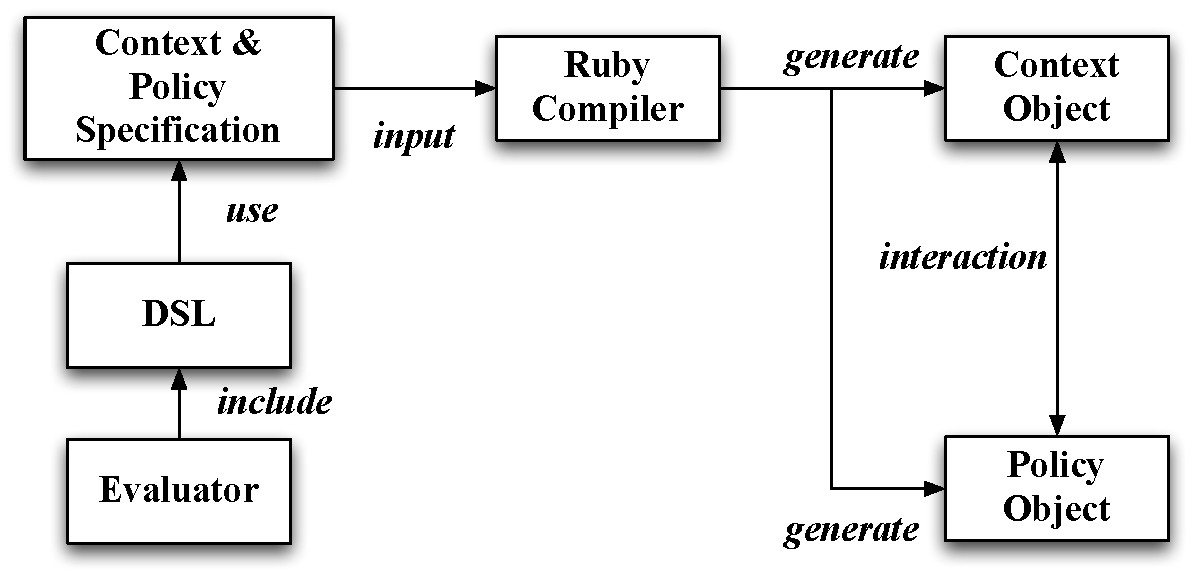
\includegraphics[width=3.5in]{DSL-usage}
\caption{The role of DSL in usage management systems}
\label{fig:DSL-usage}
\end{figure}

\subsection{Language Operation}
Figure~\ref{fig:DSL-usage} outlines the use and operation of this DSL for usage management. The DSL provides a language for specification of contexts and policies as described in the previous section. As shown in the figure, the DSL incorporates different types of evaluators for expression of different types of usage semantics. A DSL, along with an appropriate evaluator is then used to specify contexts and policies. The system as a whole allows users to choose from different types of evaluators that provide the right type of needed semantics. The policy specification and context specification, described using the DSL is then taken by a Ruby compiler to generate a corresponding context and policy object. In usage management systems, the computing platform generates and maintains context objects. The resource owners provide the policy specification, converting it into a policy object.  Following this, the policy and context objects interact with each other and operate within a usage management system.  

\subsection{Language Description}
The language is based on the model description provided in the previous section, and enables specification of the various policy semantics and context descriptions. 

\subsubsection{Context Specification}
The DSL provides a mechanism for specification of different types of contexts based on the context structure explained in the previous section. A context consists of a set of entities, such as Subject, Resource, and Environment, and each of these entities possess a set of properties. Every property supports a set of functions that operate over the property. The steps involved in defining a context first includes the description of different types of properties. The properties are then allocated to different entities, and then entities are assigned to a given context. 

\begin{table*}[t]
\caption{An example structure of context.}
\label{table:context}
\begin{center}
%{\small
\begin{tabular}{|c|c|c|c|}
\hline
\multicolumn{4}{|c|}{ \bf Context}\\
\hline
{ \bf Entity} & {\bf Property ($p$)} & { \bf Domain ($D_p$)} & {\bf Functions ($F_p$)}\\
\hline
\multirow{3}{*}{Environment (E)} & OperatingSystem & \{Windows, OSX, SELinux\}&  equatable\\
                                                    & Device & \{Workstation, Handheld, Blackberry, Terminal\} & equatable \\
                                                    & SecurityDomain & \{ ABNet, SECNet, TELNet, OMNINet\} & comparable\\ 
\hline
\multirow{3}{*}{Subject (S)} & SecurityClearance & \{Top Secret, Secret, Confidential\} &  comparable\\
				      &Project & \{Zebra, Yuma, Lion\} & equatable\\
				       &Role & \{Alpha, Beta, Delta\} & equatable\\

\hline
 Resource(R) & SecurityClassification & \{ Top Secret, Secret, Confidential, Unclassified\} & comparable \\
\hline

\end{tabular}
%}
\end{center}
\label{default}
\end{table*} 

Consider a multi-level security context as shown in Table~\ref{table:context}. The context consists of three entities, namely, {\em Subject}, {\em Environment} and {\em Resource}. The {\em Subject} entity has three properties, namely, {\em Security Clearance}, {\em Role} and {\em Project}.  The {\em Environment} entity has three properties, namely, {\em OperatingSystem}, {\em Device} and {\em SecurityDomain}.  The {\em Resource} entity has one property, {\em SecurityClassification}. Every property supports a set of functions depending on the type of that property.  For the purpose of this discussion, we explain two types of properties, namely, equatable and comparable.  Equatable properties primarily support equality functions  ``$=$" and ``$\ne$". Comparable properties support functions that allow relative comparison of two values, namely, ``$=$" , ``$\ne$", ``$<$", ``$>$",  ``$\leq$", ``$\geq$" and ``$between()$". Both equatable and comparable property types support ``$get()$" and ``$set()$" functions to retrieve and set property values. The properties {\em OperatingSystem}, {\em Device}, {\em Project} and {\em Role} are equatable properties, and {\em SecurityDomain}, {\em SecurityClearance} and {\em SecurityClassfication} are comparable properties. {\em SecurityDomain} property values have the ordering $ABNet > SECNet > TELNet > OMNINet$,  {\em SecurityClearance} property values have the ordering $Top\;Secret > Secret > Confidential$, and {\em SecurityClassification} property values have the ordering $Top\;Secret > Secret > Confidential > Unclassified$. 

In order to specify this context, individual properties are defined first: 

\lstinputlisting[]{content/code/policy/property_1.pol}
	
This example specifies classes {\em OperatingSystem, Device, Project} and {\em Role} that implement the type {\em Property}. The term {\em values} specifies the set of valid values and {\em functions} define the set of functions supported by the class as described earlier. Similarly, the system defines classes for comparable properties, with the addition that the user specifies the ordering of the valid values: 

\lstinputlisting[]{content/code/policy/property_2.pol}

Here we generate the classes {\em SecurityDomain}, {\em SecurityClearance} and {\em SecurityClassification} that implement the type {\em Property}. Each of these classes are comparable and provide a set of comparison functions. The {\em order} keyword allows context designers to specify the value ordering in an easy manner. The property classes defined here are now assigned to the entities {\em Subject}, {\em Resource} and {\em Environment}. These assignments are described in the DSL as follows: 

\lstinputlisting[]{content/code/policy/entity.pol}

The above specification generates the {\em Subject}, {\em Resource} and {\em Environment} classes. The DSL generates a {\em Subject} class that contains properties of type {\em Role}, {\em Project}, and {\em SecurityClearance}. Entity type classes, by default, implement functions that provide information about the  properties these entities contain. Finally, the context includes each of these entities, which in this case is a multi-level security context. The syntax for context specification is as follows. 

\lstinputlisting[]{content/code/policy/context.pol}

This specification generates the {\em MultilevelSecurity} class that contains entities {\em Subject}, {\em Resource} and {\em Environment}. The process of context specification is carried out by context designers. This is a less frequently carried out process, but the DSL still provides a relatively easy way to provide this specification. The {\em MultilevelSecurity} class is instantiated, and the corresponding object of this class maintained on the client system. The property values of this object define the circumstances under which activities are carried out in the client system. 

It must be noted that various kinds of properties can be described using this method. For example, properties having set-based characteristics can be defined that support set functions such as ``$in()$" to determine if a given element is a part of the set. 

The context generated in this manner is then used to define policies. The DSL provides a policy specification component that enables an easy way to specify policies. Policy specifications are read by the Ruby interpreter and converted into policy objects. For example, consider the following policy: 

{\em ``A document with a security classification greater than or equal to Secret can only be viewed by subjects working on project Yuma having security clearance greater than or equal to Secret on only Blackberry devices operating in a security domain greater than SECNet. Also, viewing can be done only after project Yuma has been project-authorized. "}

This policy is expressed in terms of the DSL in the following steps: 

\lstinputlisting[]{content/code/policy/activity_1.pol}

First an activity {\em view} is declared and associated with the constraints defined in terms of context properties.  This then becomes a {\em restricted activity}, as we have imposed contextual constraints on the activity.  It must be noted that the activities defined in the DSL are agreed upon {\em a priori} with the client system.  Now we define another activity, {\em project-authorization} along with its restrictions (or constraints):

\lstinputlisting[]{content/code/policy/activity_2.pol}

Once activities {\em restricted\_view} and {\em authorization} are defined, we can establish relationships between them. Such relationships are called usage policies, and are defined by the policy definition of the DSL. Usage semantics establish relationships among different activities along with behavioral or or history-based characteristics such as count limits on a given activity. In the present form, the DSL allows permissions, obligations and count limits. However, the DSL can be extended, and usage semantics can be added or changed by using different types of evaluators. In this example, restricted activity {\em view} is a permission, and activity {\em project-authorization} is an obligation for exercising this permission. These semantics are expressed in the DSL as follows: 

\lstinputlisting[]{content/code/policy/policy_1.pol}

The above policy specification says that the policy {\em pol} is defined using activities {\em restricted\_view} and {\em authorized}.  Activity {\em restricted\_view} is a permission that is obligated by activity {\em authorization}.  Additional usage semantics could be added to this activity, for instance count-based limits:

\lstinputlisting[]{content/code/policy/policy_2.pol}

Once the policy specification is provided to the Ruby interpreter, it converts it into a policy object. A policy object is nothing but an executable ruby object with a well-defined policy interface. An example interface provided by the standard policy evaluator defined here contains the below set of functions.

Note, in both policies we explicitly identify the constraint and policy evaluators.  This is done for clarity in this case; these values are in fact the default interpretation values used so those statements could very well be omitted.

\begin{itemize}
\item {\bf permissions?()}. Returns the set of permissions for a given policy.
\item {\bf obligations?(a)}. Returns the set of all obligations associated with a given permission. 
\item {\bf remaining\_obligations(a)}. Returns the set of remaining obligations for a given permission. 
\item {\bf remaining\_count(a)}. Returns the set of remaining count for a given permission. 
\item {\bf allowed?(a, ctx)}. A boolean function that returns {\em true/false} whether a given activity can be carried out under a given context. 
\item {\bf reset()}. Resets the policy by resetting its state. 
\end{itemize}

The policy DSL proposed here is simply a skeleton which can extended by incorporating different types of logics expressing various usage semantics. The manner in which these extensions may be carried out is described next. 

\subsection{Language Extensions}

The DSL allows inclusion of different types of evaluators that provide users with different sets of usage semantics. The evaluators provide a design space for innovation and extensibility. In the examples provided here, the evaluators used for evaluating constraint (or restriction) semantics are {\em propositional} evaluators, our current default type. This type of evaluator allows constraints to be expressed as boolean formulas constructed from property functions. This evaluator provides a design space for expressing restrictions in terms of context properties. This evaluator is merely a plugin that can be replaced by a different constraint evaluator that allows constraints to be expressed in a different manner. 

Similarly, the policy construct uses a policy evaluator for expressing and reasoning about usage semantics. The {\em standard} evaluator used here allows expression of permissions, obligations and count-based limits. The usage semantics is similarly a design space where different types of evaluators can be used to express various types of usage semantics such as parallel actions, partial ordering, and interleaving semantics.

In the next section we show how different rights expression languages and frameworks such as ODRL, XrML and creative commons can be mapped to this DSL. 